\section{Visualisation}
Our goal is to design an interactive visualisation system on top of the structured prediction framework.
Figure~\ref{fig:overview} shows the overview of a live demo system, which consists of five major components: a map to display the suggested routes, an input box for user query (upper left), a stacked score of routes (upper right), a POI list box (lower left), and a radar chart to compare features of multiple POIs (lower right). 
The role and the construction of the four major components, besides the main map, are as follows:

%\begin{itemize}
\textbf{Query input}: A query consists of a starting POI and a trip length. 
Users can choose the starting POI by clicking icons on the map and can adjust the slide to set the trip length. 
In addition, three different travelling modes (e.g. bicycling, driving and walking) are supported, 
and we optimise the suggested routes for each mode.

\textbf{Route score visualisation}: 
The SSVM evaluates relevance scores of POIs and transitions in a candidate route to the given query and uses the sum of the relevance scores to determine the ranks of the routes.
To visualise the POI and transition scores, we adopt a stacked bar representation~~\cite{gratzl2013lineup}, designed to support the visualisation of multi-attribute ranking.
In Figure~\ref{fig:stack}, the system decompose the scores of top 10 recommended routes into POI and transition scores via the stacked bar representation, where the size of each bar is proportional to the relevance score of the corresponding POI and transition in the route.
Note that the POI and transition scores are scaled differently to support better visual discrimination\footnote{See Appendix for details at \url{http://arxiv.org/abs/1707.01627}}.
For a seamless match between a route on the map and the corresponding POI scores in the bar plot,
we use the same colour for both POI score and POI icon on the map.
We also allow users to select multiple rows to visualise the corresponding routes on the map.
%For each POI score, we also keep the same POI colour used to represent the POI on the map to support matching between a route on the map and bar plot seamlessly.

%Ranks of candidate routes are determined by their total scores from the SSVM. 
%The score of each route are decomposed into a set of scores for POIs and transitions along the route. 
%We adopt the LineUp framework~\cite{gratzl2013lineup} designed to support the visualisation of multi-attribute ranking via stacked representation. 
%To assist visualisation, both the POI and transition scores are properly scaled (see Appendix\footnote{https:arxiv.org/abs/???.????} for details).
%Figure~\ref{fig:stack} shows the stacked bars of the top 10 scored routes.
%Scores of different POI and transition are shown in different colours,
%and the proportion of each bar indicates the importance of the corresponding POI and transition in the route.
%At the left side, % of this representation,
%the user can select one or more suggested routes to get the numerical scores of POIs and transitions.
%All selected routes are drawn on the map, and the POIs in the most recent chosen route are shown with labelled icons.

\textbf{POI list}:
The POI list box provides the list of POI names and categories along the recommended route.
%Users can select one or more suggested routes to get more detailed information. 
%Specifically, information about the sequence of POIs in the selected route is provided, including POI names and their categories (e.g. Parks, Entertainment).
The list is sorted according to the suggested visiting order, and again, the same POI colour is used to match the corresponding POI on the map.
On top of the list, the system also provides an estimated travel time and total distance of the route. 
The POI list box is updated whenever a user selects a different route or the system makes a new recommendation. % a new route given a query.
%The list box also provides the estimated time and distance of the selected route at the top of the list.
If more than one route is selected, the system displays the information of the most recent chosen route.

\textbf{POI feature visualisation}: We further provide a radar chart to analyse the variation between POIs in a single route. 
For example, in Figure~\ref{fig:radar}, we compare two POIs (\textit{Melbourne Aquarium} and \textit{Queen Victoria Market}) in terms of POI features and their importance in the suggested route. 
The radar chart shows the corresponding POI feature scores when a user selects a route.
In particular, the user can check/uncheck any POI in the selected route, and the feature scores of all checked POIs will be shown in the chart.
%\end{itemize}

\begin{figure}[t!]
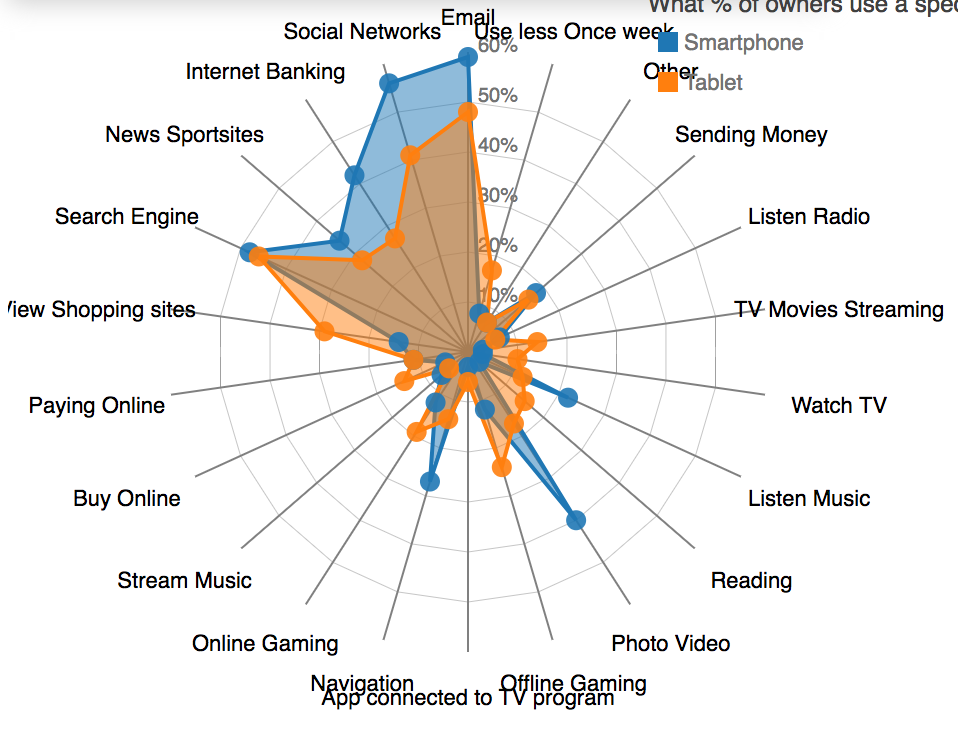
\includegraphics[width=0.6\linewidth]{figure/sample_radar.png} \vspace{-10pt}
    \caption{POI feature comparison between \textit{Melbourne Aquarium} and \textit{Queen Victoria Market}: the former scores higher on \textit{Popularity} and \textit{Visits difference} features whereas the latter scores higher on \textit{Visits} and \textit{Popularity difference} features.}
\label{fig:radar} \vspace{-1em}
\end{figure}
